\begin{frame}
    \frametitle{Separar datos del código}

        %En todo momento se ha procurado separar todos los datos de los personajes, circuitos y menús, del código
        %fuente.\\
        Desacople código / datos (personajes, circuitos, menús, etc).\\
        \begin{block}{Ventajas}
            \begin{itemize}
                \item No es necesario saber programar para realizar cambios sobre cualquier parámetro
                \item Cualquier persona puede ampliar el juego con nuevos personajes y nuevos circuitos, siguiendo
                los manuales creados para ello
            \end{itemize}
        \end{block}
        \begin{block}{Solución}
            \begin{itemize}
                \item Todo se lee de ficheros XML
            \end{itemize}
        \end{block}

        \begin{center}
                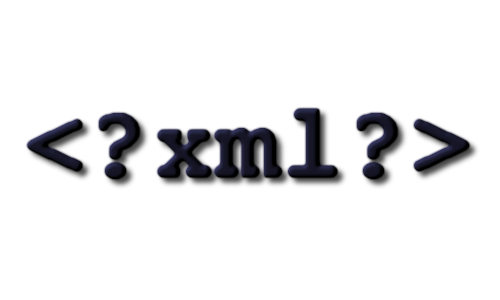
\includegraphics[scale=0.25]{imagenes/logo_xml.png}
        \end{center}

\end{frame}

\begin{frame}
    \frametitle{Formato de circuitos}

    \begin{block}{Mapas de tiles}
        Tile: imagen cuadrada usada para generar imágenes de mayor complejidad.\\
        Usor del editor de mapas Tiled.
    \end{block}   
    
    %\begin{block}{Editor de mapas: Tiled}
    %Proporcionaba todas las necesidades básicas, 
    %como una sencilla edición y creación de niveles, así como la gestión de capas,
    %para poder poner elementos en el circuito a un nivel superior o inferior.\\
    %Para ello se debía crear una imagen con todos los tiles que compondrían un circuito (tileset).\\
    %Genera como resultado un XML.
    %\end{block}   

        \begin{center}
                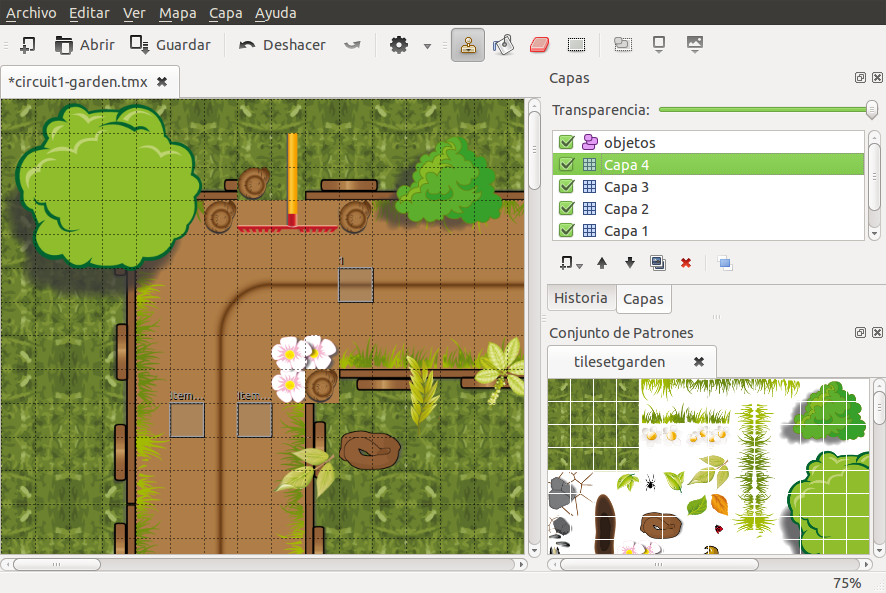
\includegraphics[scale=0.28]{imagenes/captura_tiled.png}
        \end{center}


\end{frame}

\begin{frame}
    \frametitle{Formato de circuitos}

    \begin{columns}

        \column{150px}

        \begin{block}{Inconveniente}
            %No permite indicar de forma sencilla que tiles eran atravesables, colisionables o de cualquier otro tipo.
            No permite indicar los tipos de los tiles.
        \end{block}
    
        \begin{block}{Solución}
        %Una imagen extra con las mismas características, donde los tiles sera de un único color, en función del tipo
        %que estos sean.
        Usar una imagen extra.
        \end{block}

        \column{180px}
        \begin{center}
                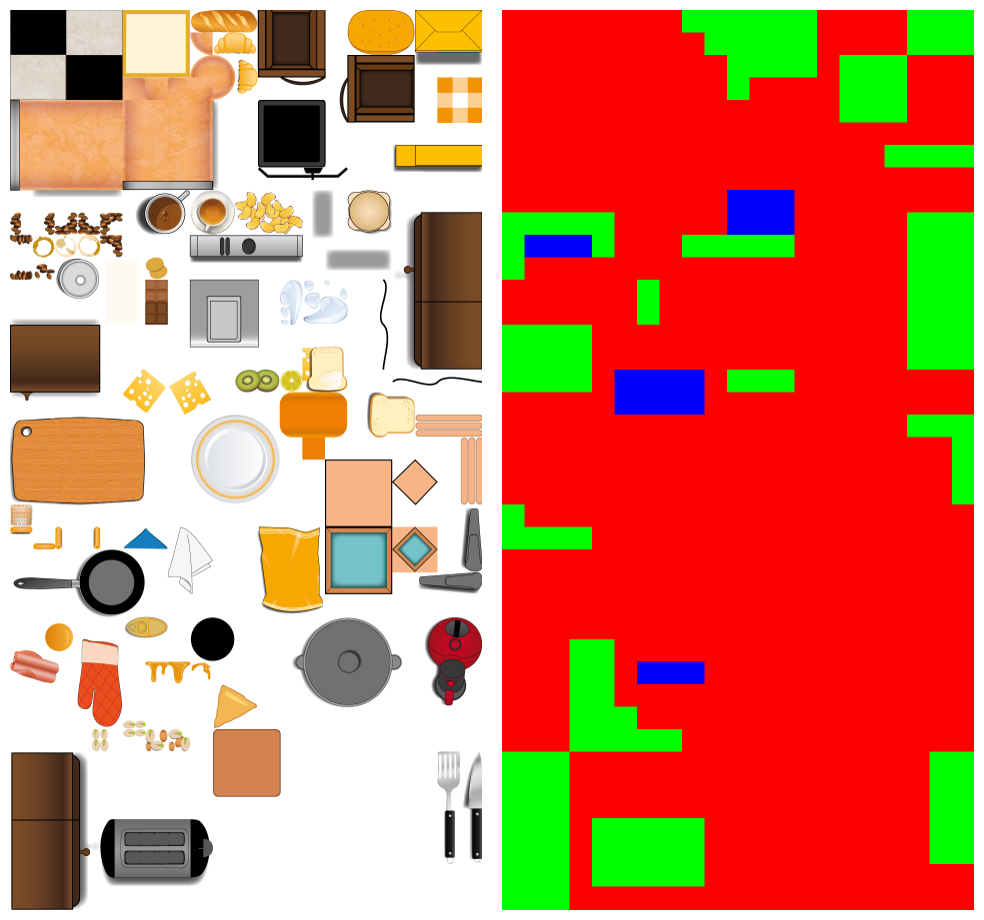
\includegraphics[scale=0.18]{imagenes/tileset-collisionmap.png}
        \end{center}
        
    \end{columns}

\end{frame}

\begin{frame}
    \frametitle{Colisiones}
    
    Una de los aspectos más importantes en este tipo de juegos.
    \begin{block}{Colisión con el escenario}
        \begin{itemize}
            \item Detectamos si atravesamos algún tile no atravesable
            \item Si es así corregimos la posición del coche en según la dirección, sentido y lado del tile por
            el que colisione
            \item En el caso de que el tile sea de tipo ralentizador, diminuimos la velocidad del coche
        \end{itemize}
    \end{block}

    \begin{center}
        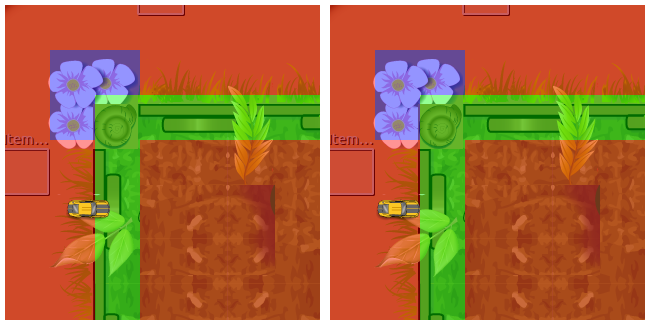
\includegraphics[scale=0.3]{imagenes/colision1-colision2.png}
    \end{center}
\end{frame}

\begin{frame}
    \frametitle{Colisiones}
    
    \begin{block}{Colisión entre vehículos}
        \begin{itemize}
            \item De forma similar a la colisión con el escenario
            \item Cuando se detecta la colisión se corrige la posición de los vehículos, en función la dirección, 
            sentido y lado por el que colisionen
            \item Podemos usar nuestro coche para evitar adelantamientos
        \end{itemize}
    \end{block}
    
    \begin{block}{Colisión con ítems de ataque}
      \begin{itemize}
            \item Se destruye el ítem y se cambia el estado del coche que colisiona
        \end{itemize}
    \end{block}
    
    \begin{block}{Colisión con obstáculos}
      \begin{itemize}
            \item Cambia el estado del coche en función del tipo de obstáculo (atravesable o no)
        \end{itemize}
    \end{block}

\end{frame}

\begin{frame}
    \frametitle{Inteligencia artificial}
    %Otro de los aspectos más importante de un videojuego de las características de Zycars, es la
    %inteligencia artificial, ya que en dos de los tres modos de juegos disponibles el objetivo es obtener la
    %mejor clasificación posible, por delante de los demás coches controlados por el ordenador
    Aspectos muy importante en videojuego de las características
    de Zycars: interviene en en dos de los tres modos de
    juegos.

        \begin{block}{Habilidades}
            \begin{itemize}
                \item Realización del recorrido: debe ser capaz de realizar los 
                recorridos de los circuitos
                \item Lanzamiento de ítems: también debe poder usar los ítems que reciba de las bolas de ítems
            \end{itemize}
        \end{block}
        
        \begin{center}
                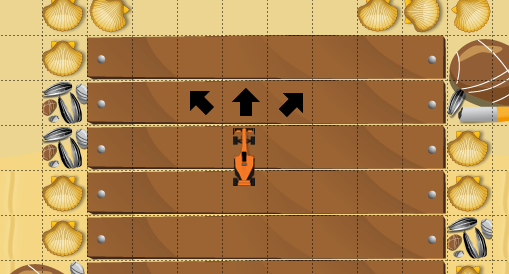
\includegraphics[scale=0.5]{imagenes/ia2.png}
        \end{center}
        

        
\end{frame}

\begin{frame}
    \frametitle{Realización del recorrido. Algoritmo A*}

    %Aprovechando que tenemos un circuito creado por tiles y que podemos saber en todo momento en el tile 
    %actual que se puede encontrar cualquiera de los competidores, se decidió implementar el 
    %algoritmo de búsqueda A*.
    
    Teniendo un circuito de tiles podemos realizar búsquedas de caminos a través de estos.

        \begin{block}{Objetivo}
        Buscar el camino más corto y óptimo desde
        un nodo origen, hasta un nodo destino. Se tienen en cuenta factores
        como el valor heurístico de los nodos, así como el coste real del recorrido.
        \end{block}

        \begin{block}{Parámetros}
        Los parámetros que se tienen en cuenta en la búsqueda:
            \begin{itemize}
                \item h’(n) es el valor heurístico del nodo actual n, hasta el final
                \item g(n) el coste real del camino desde el origen al nodo actual
                \item Función de evaluación: f(n) = g(n) + h’(n)
            \end{itemize}
        \end{block}

        \begin{block}{Estructuras}
            \begin{itemize}
                \item Lista de abiertos: nodos por los que aún no se han pasado
                \item Lista de cerrados: nodos por los que ya se han pasado
            \end{itemize}
        \end{block}
        
\end{frame}

\begin{frame}
    \frametitle{Realización del recorrido. Algoritmo A*}

    %\begin{columns}
    
        %\column{200px}
        \begin{block}{Funcionamiento}
            Partiendo del nodo actual:
            \begin{enumerate}
                \item Obtenemos vecinos
                \item Si no están en abiertos ni cerrados y los metemos en abiertos
                %\item Si alguno esta en abiertos, comprobamos su f(n), si es menor lo sustituiremos
                %\item Introducimos en abiertos los que cumplan las condiciones
                \item Obtenemos de abiertos el nodo con menor f(n) y comenzamos de nuevo 
                \item Una vez en el nodo objetivo, detenemos la búsqueda y devolvemos el camino
            \end{enumerate}
        \end{block}
        
        %\column{150px}
        \begin{center}
                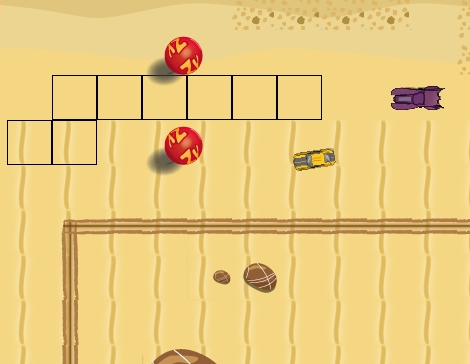
\includegraphics[scale=0.3]{imagenes/a*_ejemplo.png}
        \end{center}
    
    %\end{columns}

\end{frame}

\begin{frame}
    \frametitle{Lanzamientos de ítems}

    Capaz de lanzar los ítems disponibles a los largo del juego, según las
    distintas situaciones en la que se encuentre.

        \begin{block}{Solución}
        Cada vehículo tiene dos segmentos:
            \begin{itemize}
                \item Delantero: comprueba si algún oponente está delante para lanzar ítem
                \item Trasero: verifica la parte trasera en busca de algún oponente para dejar un obstáculo
            \end{itemize}
        %uno desde el centro delcoche hacia unos píxeles por delante su posición y otro desde el centro uno píxeles atrás de la posición.
        \end{block}

        \begin{center}
                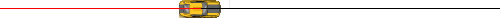
\includegraphics[scale=0.5]{imagenes/ia_segmentos.png}
        \end{center}

        \begin{center}
                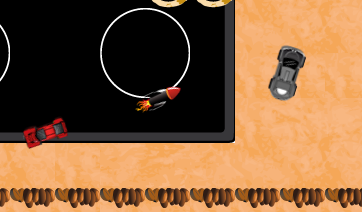
\includegraphics[scale=0.5]{imagenes/ia_lanzar.png}
        \end{center}
\end{frame}

\begin{frame}
    \frametitle{Recopilación}

    \begin{columns}
    
        \column{200px}
        \begin{block}{Zycars}
            \begin{itemize}
                \item Multiplataforma
                \item 12 circuitos
                \item 3 modos de juego
                \item 3 campeonatos
                \item 7 personajes
                \item 6 ítems
                \item Circuitos ampliables con tiled
                \item Personajes ampliables
                \item Dificultad adecuada
            \end{itemize}
        %uno desde el centro delcoche hacia unos píxeles por delante su posición y otro desde el centro uno píxeles atrás de la posición.
        \end{block}

        \column{100px}
        \begin{center}
                
\includegraphics[scale=0.5]{imagenes/character2.png}
        \end{center}
    
    \end{columns}
        
\end{frame}
